\chapter{Desenvolvimento\label{ch:develop}}

\begin{flushright}
\textit{Simple, clear purpose and principles give rise to complex, intelligent behavior. Complex rules and regulations give rise to simple and stupid behavior.}\\(Hock Dee)
\end{flushright}

Em trabalhos anteriores foram propostos e implementados vários controladores cinemáticos como forma de corrigir o efeito das pertubações devido a interação com uma agente externo e da ação da gravidade. No entanto o desempenho foi abaixo do apresentado pela código de demonstração do fabricante para o robô e pelos mesmos controladores no uso em outra plataforma explicitando a necessidade de um maior estudo da arquitetura do manipulador robótico Meka A2. Com base nisto foi feito uma análise do componentes do braço e a implementação dos sistemas de controle das juntas em software e hardware. Neste capítulo será descrito os métodos de investigação utilizados bem como experimentos efetuados.

\section{Avaliação de Desempenho}

Em \cite{nocite} Marcos propôs diversas métricas e avaliar os controladores cinemáticos implementados. Enquanto foi possível um excelente detalhamento da desempenho comparativa de cada um dos controladores, foi descoberto limitações na interação com a plataforma. Neste trabalho será analisado o robô enquanto sistema observando as implicações dos componentes mecânicos, software e sistemas de controle operando de forma conjunta. O objetivo é avaliar dentro do que já foi implementado os limites de desempenho permitidos pela plataforma para permitir um melhor desempenho em trabalhos futuros. 

\begin{figure}[H]
    \centering
    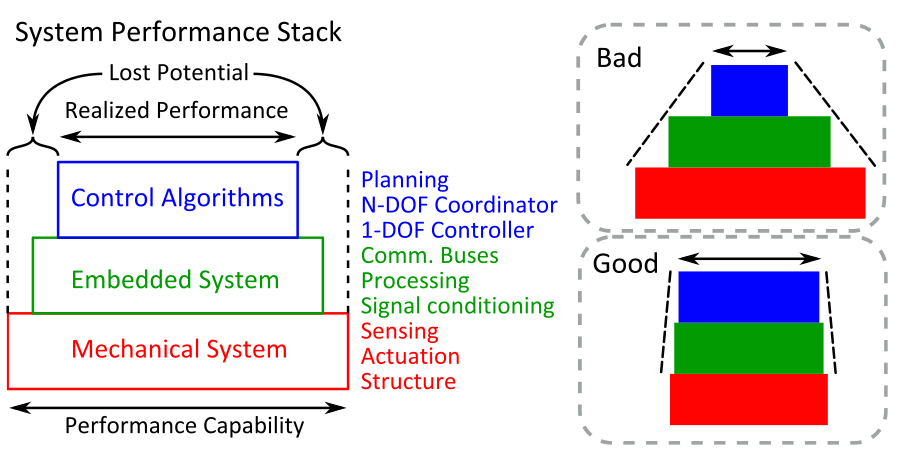
\includegraphics[width = \linewidth]{tex/figs/system_perfomance.png}
    \caption{Representação do Desempenho de um sistema \cite{paine2014high}}
    \label{fig:system_perfomance}
\end{figure}

Por se tratar de um sistema mecatrônico, naturalmente existem 3 camadas: Sistema Mecânico, Sistema Embarcado e Algorítimos de Controle conforme ilustrado na figura \ref{fig:system_perfomance} proposta por N. A. Paine em \cite{paine2014high} para o desenvolvimento de um sistema série elástico de alta performance. Para o Meka estas camadas estão implementados na seguinte forma:

\begin{itemize}
    \item Sistema Mecânico ( Atuadores Série Elásticos )
    \begin{itemize}
        \item Motores Brushless
        \item Harmonic Drive
    \end{itemize}
    \item Sistema Embarcado ( Atuadores Série Elásticos )
    \begin{itemize}
        \item Placa DSP para controle dos motores
        \item Hub EtherCAT
        \item Interface EtherCAT para o computador
        \item PC com Linux Ubuntu 12.04 e Kernel RTOS Xenomai
    \end{itemize}
    \item Algoritmos de Controle
    \begin{itemize}
        \item Controle de Torque (DSP)
        \item Controle de Posição com Compensação da Gravidade (PC)
        \item Interface ROS
        \item Controle Cinemático
        \item Gerador de Trajetória
    \end{itemize}
\end{itemize}

Como forma de alcançar um maior desempenho com o Meka foram avaliadas cada parte quanto a possíveis limitações e assim orientar trabalhos futuros no controle do robô.

% Comentar sobre desempenho de sistemas
% - Como alcançar o maior desempenho do sistema ( Custo exponencial 99.9 )
% - Não linearidades identificadas

% Avaliação Sistema Mecânico
% - Estudo SEA
% - Documentação
% Avaliação Sistema Embarcado?
% - Documentação EtherCAT, RTOS, PC
% - Tempo de Resposta da Comunicação
% Avaliação Controle
% - Ensaios Estabilidade em Malha Fechada
% - Ensaios em Degrau

% TODO Colocar nos resultados:
%No qual foi observado que aspectos particulares da plataforma não foram levados em conta como a operação em regiões não lineares do sistema devido a saturação da velocidade e torque dos motores, tempos longo de atraso de comunicação entre o computador.

% Reprodução Resultados Marcos

\section{Avaliação Preliminar}

Inicialmente foi feito um estudo a partir do código de demonstração do fabricante feito em Python para avaliar quais as possíveis forma de controlar o braço. Em que foi levantando todos os controladores implementados na biblioteca m3 e testados individualmente através da API em Python. Estão disponíveis os seguintes controladores pela biblioteca:

\begin{itemize}
    \item Controle de Posição
    \item Controle de Posição com compensação da gravidade
    \item Controle de Torque
    \item Controle de Torque com compensação da gravidade
    \item Controle de Velocidade
\end{itemize}

%Nesta avaliação foi notado que alguns dos controladores da m3 não estavam disponíveis nas interfaces em C++. 

Para análise do comportamento em conjunto dos controladores cinemáticos foi definido o controlador de posição com compensação da gravidade, uma vez que este que é usado pela ROS.

\section{Estudo Controladores Cinemáticos}

Para definir um ponto de referência para os ensaios e testes, foram avaliados os controladores implementados por Marcos Pereira. A partir da melhor configuração para cada um dos controladores foram feitos experimentos ajustando os parâmetros da velocidade de atuação e nível rigidez para avaliar a influência nos resultados. Os experimentos foram executados foram feitos com base em duas trajetórias pré-definidas: deslocamento em linha reta na vertical e o desenho de um quadrado a partir de dois deslocamentos na vertical e dois na horizontal.

Nos experimentos de deslocamento em linha reta foram avaliados o intervalo de tempo até robô começar a responder e o controle estabilizar para diferentes taxas de amostragem da trajetória. Enquanto nos experimentos com a trajetória de quadrado foram avaliadas a resposta do robô para diferentes valores de ajuste dos controladores de junta quanto aos parâmetros de velocidade e rigidez.

\subsection{Avaliação tempo de amostragem}

Para avaliar os tempos de atuação foi repetido o mesmo experimento para o deslocamento em linha reta na vertical. Neste experimento foi estudado o tempo necessário para o atuador começar a se mover dado um comando bem o tempo necessário para o controle convergir.

% Resultados

\subsection{Estudo Interação do controle de rigidez}

\section{Layout Experimentos}

Para avaliar a resposta do sistema para controle dos ângulos de junta foi proposto um teste com estímulo pelo degrau. Esta avaliação foi efetuada para interação pela API em Python e pelo ROS. Para ambos casos os dados obtidos foram registrados em arquivo utilizando a ferramenta rosbag. 

% Comentar sobre como a informação é publicada nos tópicos

% Levantamento dos problemas

% Investigação de possíveis causas


\subsection{shm\_humanoid\_interface}

Este é um nó do ROS disponibilizado pela Meka Robotics para a comunicação via ROS com o Meka. Representa uma das possíveis interfaces com a M3 através do acesso direto a memória compartilhada. Através deste nó são gerados dois tópicos no ros: $/humanoid\_state$ e $/humanoid\_command$. A cada interação a informação atual do tópico $/hummanoid_command$ é passada para a memória compartilhada e a leitura dos sensores é então escrita no tópico $/hummanoid_state$. Na versão atual são somente interpretados os comando de posição das juntas através dos modos de controle com e sem compensação da gravidade.

\subsection{ROS Bags}

ROS Bags é um utilitário do ROS para o registro dos eventos em cada tópico. A informação publicada nos tópicos é registrada em formato yaml e permite que que posteriormente possa ser reproduzida em tópicos tal uma simulação. Desta forma dispensa a necessidade de manter o hardware conectado para analisar o comportamento do robô ao longo do tempo bem como permitir a análise de diferentes experimentos diretamente pelas ferramentas do ROS como o \textit{ros\_plot}. Ou ainda conectar os resultados de um hardware real com uma simulação como forma de efetuar uma validação cruzada do comportamento real em comparação do comportamento simulado. Para tal basta executar o programa e indicar quais tópicos serão monitorados. Ao final da execução é registrado um arquivo com as informações com a extensão $.bag$. Internamente os dados são registrados em formato $.yaml$ o que permite a leitura direta.

No entanto a representação da informação é um pouco verbosa gerando um arquivo grande. Assim foi utilizado o programa $bag2csv$ para converter para o formato $.csv$ para facilitar o processamento. Em seguida o programa $sed$ para pequenos ajustes e a separação da leitura dos tópicos  $/humanoid\_state$ e $/humanoid\_command$ em diferentes arquivos. Este processo foi incorporado a Makefile para permitir o processamento rápido de todos os arquivos $.bag$ utilizando o recurso de processamento paralelo da ferramenta GNU make\footnote{\url{https://www.gnu.org/software/make/manual/html_node/Parallel.html}}.

\subsection{Python API}

Além do controle via ROS, a M3 possui uma interface através de uma API em Python que permite uma liberdade maior de controle uma vez que possui mais recursos já implementados. Além do modos de controle por posição estão também disponíveis o controle direto por torque e por velocidade das juntas. Estão implementados um controlador para compensação do efeito da gravidade a partir da biblioteca KDL com base no momento de inércia de cada junta.

% Explicação sobre funcionamento da biblioteca
% Diagrama: Comando/Estado -> Memória "bot" -> "proxy.step()"
% -> Problema Detectado no uso do ângulo em radianos por isto foi adotado o uso em graus